%
% THE BEER-WARE LICENSE (Rev. 42):
% Ronny Bergmann <bergmann@math.uni-luebeck.de> wrote this file. As long as you
% retain this notice you can do whatever you want with this stuff. If we meet
% some day, and you think this stuff is worth it, you can buy me a beer or
% coffee in return.
%
% This file is just to get started - You need the corresponding Logo
%
\documentclass[german,10pt,xcolor=colortbl,compress]{beamer}
\usepackage[utf8]{inputenc}
\usepackage[ngerman]{babel} % Neue Rechtschreibung
\usepackage{amsmath,amsthm,amssymb,euscript} % AMS-LaTeX  
\usepackage{enumerate,graphicx}

\usepackage{tikz}

\usepackage[separate-uncertainty = true,multi-part-units=single]{siunitx}
\sisetup{
	locale = DE,
	%allow-number-unit-breaks,
	tight-spacing
}

\setbeamerfont{footnote}{size=\tiny}
\def\Put(#1,#2)#3{\leavevmode\makebox(0,0){\put(#1,#2){#3}}}

\usepackage{pgfpages}
%\setbeameroption{show notes}
%\setbeameroption{show notes on second screen=right}

% ~ TODO command
\newcommand{\TODO}[1]{\textcolor{red}{(TODO #1)}} % Markierung von TODOs im Text

% Load Them
\usetheme[slogan=false, navigation=true,reducedframetotal, myriad=true]{UzL}
%
\setbeamertemplate{navigation symbols}{}
\title{Projektpraktikum Robotik und Automation:\\Künstliche Intelligenz}
\date[]{\today}
\author[Team $m^2$]{Team $m^2$: Marius Krusen und F. J. Michael Werner}
% Clear Logo 1 to make the head smaller
\institute[Universität zu Lübeck]{ROB}
\clearlogo{1}
\setlogo{1}{.25\paperwidth}{logos/Logo_Uni_Luebeck_300dpi.png}%

\definecolor{green}{RGB}{149,188,14}
\definecolor{red}{RGB}{181,22,33}
\definecolor{blue}{RGB}{0,75,90}
\definecolor{yellow}{RGB}{250,187,0}
\definecolor{orange}{RGB}{236,116,4}
\definecolor{brown}{RGB}{129,53,19}
\definecolor{uzlgreen}{RGB}{129, 53, 19}

%\setbeamerfont{caption}{size=\footnotesize}
\setbeamercolor{sectionframe}{fg=uzlmain,bg=white}
%-------------------------------------
% Titelfolie für neues Kapitel
%-------------------------------------
\AtBeginSection[]{
	\setbeamertemplate{footline}[UzLplain]
	\begin{frame}
		\vfill
		\centering
		\begin{beamercolorbox}[sep=8pt,center,shadow=true, rounded=true]{sectionframe}
			\usebeamerfont{title}\huge{\insertsectionhead}\par%
		\end{beamercolorbox}
		\vfill
	\end{frame}
	\setbeamertemplate{footline}[UzL]
	\addtocounter{framenumber}{-1}
}

\newboolean{longversion}
\setboolean{longversion}{false}

\begin{document}
	\maketitle
	\section{NEAT}
	\frame{
	\textbf{NeuroEvolution of Augmenting Topologies (NEAT)}
	\centering
	\begin{figure}
		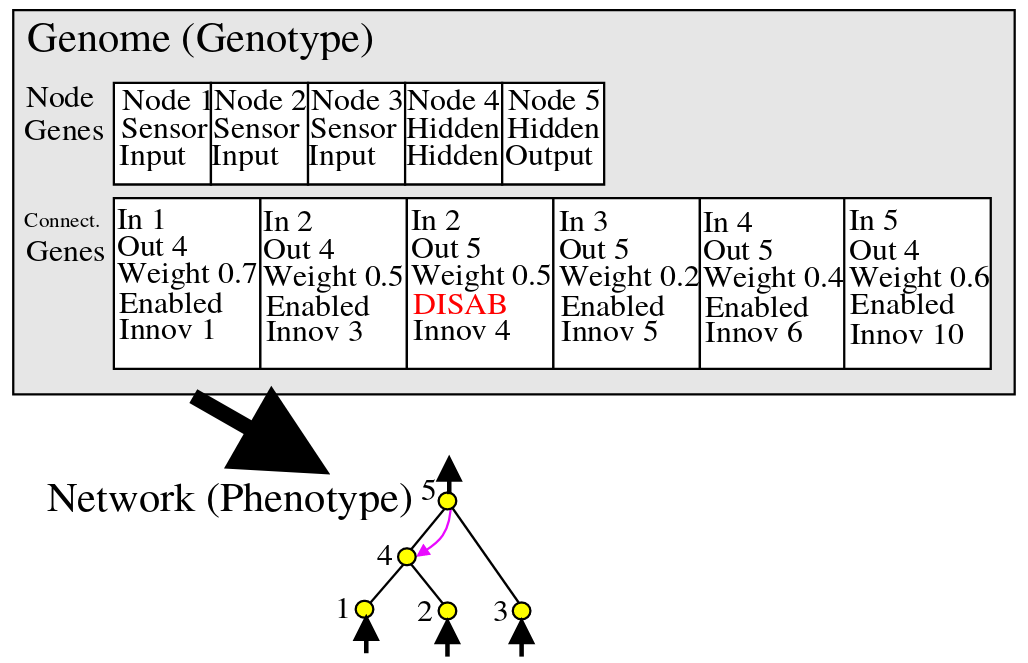
\includegraphics[width=0.75\textwidth]{images/neat_encoding.png}
	\end{figure}
	}

	\frame{
	\textbf{NeuroEvolution of Augmenting Topologies (NEAT)}
	\centering
	\begin{figure}
		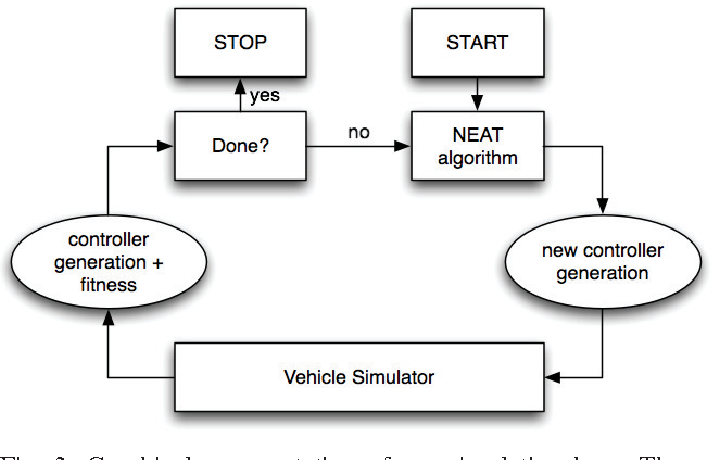
\includegraphics[width=\textwidth]{images/NEAT.png}
	\end{figure}
	}

		\frame{
		\textbf{NeuroEvolution of Augmenting Topologies (NEAT)}
		\centering
		\begin{figure}
			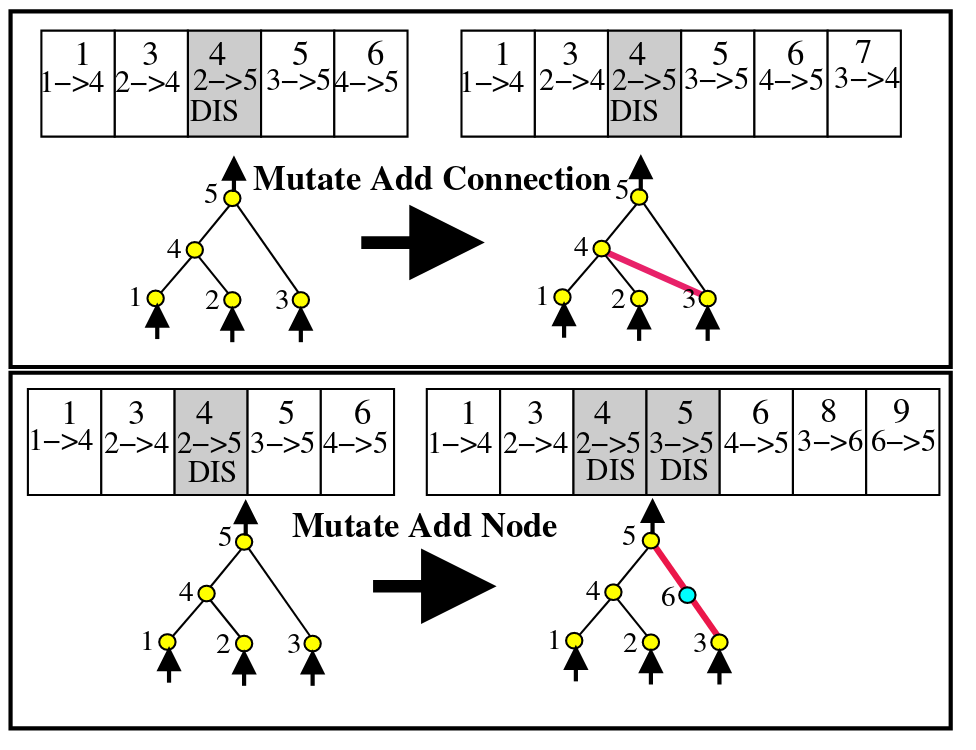
\includegraphics[width=0.75\textwidth]{images/NEAT_mutation.png}
		\end{figure}
	}

	\section{Merkmale}
	\frame{
		\textbf{Input}
		\begin{itemize}
			\item Geschwindigkeit in x- und y-Richtung
			\item Abstand zu Kontrollpunkten in x- und y-Richtung
			\item Abstand zu dem nächsten Hindernis in Fahrtrichtung
		\end{itemize}
		\vspace{0.5cm}
		\textbf{Output}
		\begin{itemize}
			\item Variante 1: 4 Ausgaben für jede Richtung
			\item Variante 2: 2 Ausgaben für jeweils vertikal und horizontal
		\end{itemize}
	}

	\section{Streckenerkennung}
	\frame{
		\textbf{Streckenerkennung}
		\\\ \\
		\begin{minipage}{0.5\textwidth}
		\begin{figure}
			\centering
			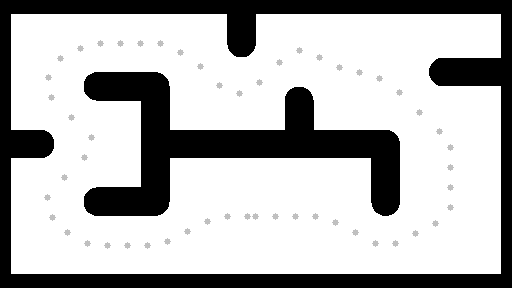
\includegraphics[width=0.95\columnwidth]{images/watershed_result.png}
			Watershed-Algorithmus
			\label{fig-watershed}
		\end{figure}
		\end{minipage}%
		\begin{minipage}{0.5\textwidth}
		\begin{figure}
			\centering
			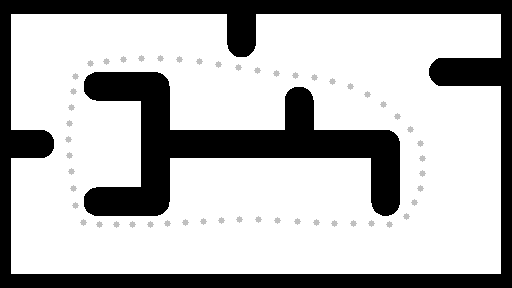
\includegraphics[width=0.95\columnwidth]{images/snake_result.png}
			Snake-Algorithmus
			\label{fig-snake}
			\end{figure}
			\end{minipage}		
	}

	\section{Merkmalsberechnung}
	\frame{
		\textbf{Position}
		\begin{itemize}
			\item Schwellenwertverfahren zur Filterung der Ballfarbe
			\item Mittelung aller verbleibenden Pixel
		\end{itemize}
		\textbf{Geschwindigkeit}
		\begin{itemize}
			\item Differenz der Positionen über sieben Frames
		\end{itemize}
		\textbf{Abstände}
		\begin{itemize}
			\item Hindernis
			\begin{itemize}
				\item Pixelweise Überprüfung entlang Fahrtrichtung
				\item Wände und Gegner
			\end{itemize}
			\item Kontrollpunkte
			\begin{itemize}
				\item Karte, die jedem Pixel nächsten Kontrollpunkt zuweist
				\item Abstand von aktueller Position zu nächstem Kontrollpunkt
			\end{itemize}
		\end{itemize}
	}

	\section{Experimente}
	
	\begin{frame}
	\textbf{Experimente und Ergebnisse}
		\begin{figure}
			\centering
			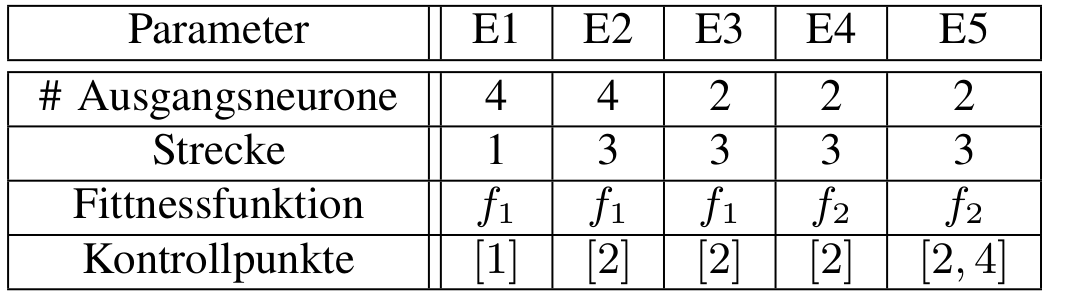
\includegraphics[width=0.65\columnwidth]{images/exp_parameters.png}
			\label{fig-watershed}
		\end{figure}
		
		\begin{figure}
			\centering
			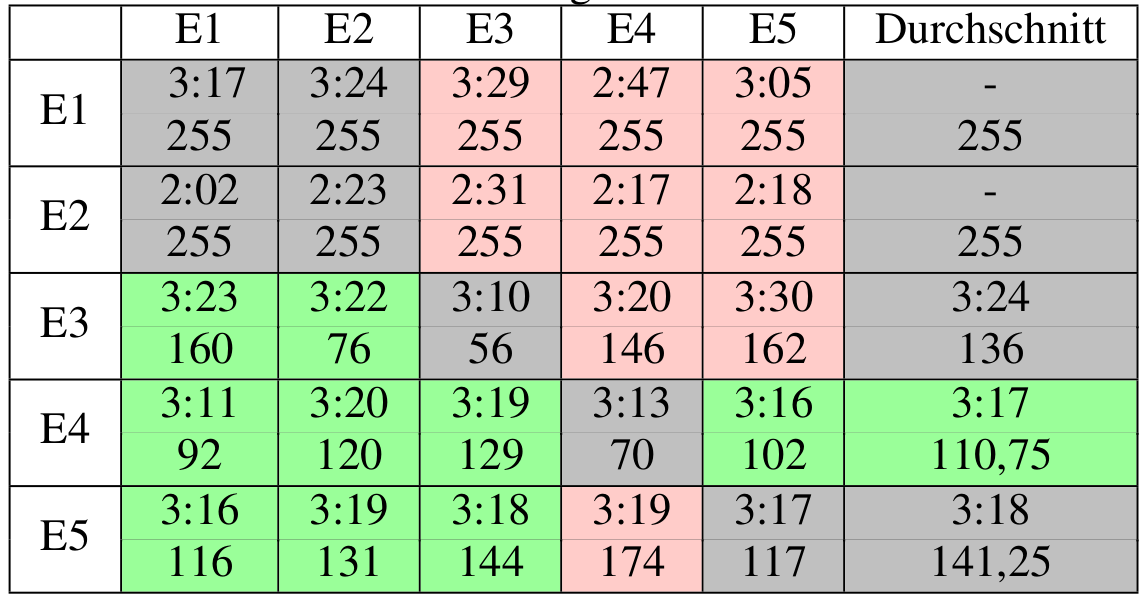
\includegraphics[width=0.65\columnwidth]{images/exp_results.png}
			\label{fig-watershed}
		\end{figure}
		
	\end{frame}

	\begin{frame}
		\textbf{rAIcer-Winner}
		\begin{figure}
			\centering
			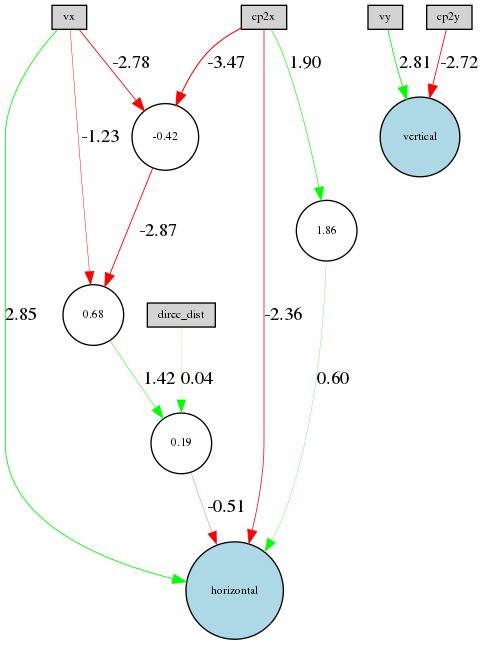
\includegraphics[height=0.8\textheight]{images/winner_e4_clean.png}
		\end{figure}
\end{frame}

\end{document}